\section{Neural Light Cones}

The concept of neural light cones provides a powerful framework for understanding how conscious experience maintains coherence while remaining bounded by physical constraints. Drawing inspiration from relativistic physics, where light cones define the possible causal relationships between events in spacetime, neural light cones describe the regions of the brain that can maintain causal connectivity and energetic coherence within the temporal windows required for conscious processing \cite{herzog2016time}.

Just as a light cone in physics determines which events can causally influence each other given the speed of light, a neural light cone defines the spatial and temporal boundaries within which brain regions can achieve the coherent energy dynamics necessary for conscious experience \cite{northoff2017how}. This bounded region is determined by several factors: the propagation speed of neural signals, the maintenance of energetic coherence, and the thermodynamic constraints on information integration \cite{bekenstein1981universal}.

Within a neural light cone, energy flows must maintain sufficient coherence to support conscious processing. This requires a delicate balance between stability and adaptability, achieved through the continuous interaction of multiple mechanisms. Neurons and astrocytes within the cone maintain synchronized activity patterns, while gap junctions and synaptic connections enable rapid signal propagation that preserves informational and energetic coherence \cite{melloni2007synchronization}. The boundaries of the neural light cone are not fixed but dynamic, shifting based on metabolic conditions, attention, and task demands.

Critically, the neural light cone concept helps explain why consciousness cannot extend arbitrarily across space and time. Just as physical causality is limited by the speed of light, conscious integration is limited by the speed of neural signal propagation and the maintenance of energetic coherence \cite{delcul2007brain}. This explains why, for instance, widely separated brain regions cannot achieve direct conscious integration without intermediate processing steps, and why consciousness requires a minimum temporal window for integration.

The neural light cone framework also provides insight into the structure of conscious experience. Regions within the cone can maintain the coherent energy dynamics necessary for conscious processing, while areas outside the cone may support cognitive function without directly contributing to conscious experience \cite{zylberberg2010brain}. This selective inclusion in consciousness is not arbitrary but follows directly from the physical constraints on maintaining energetic coherence across neural networks.

\begin{figure}[h]
    \centering
    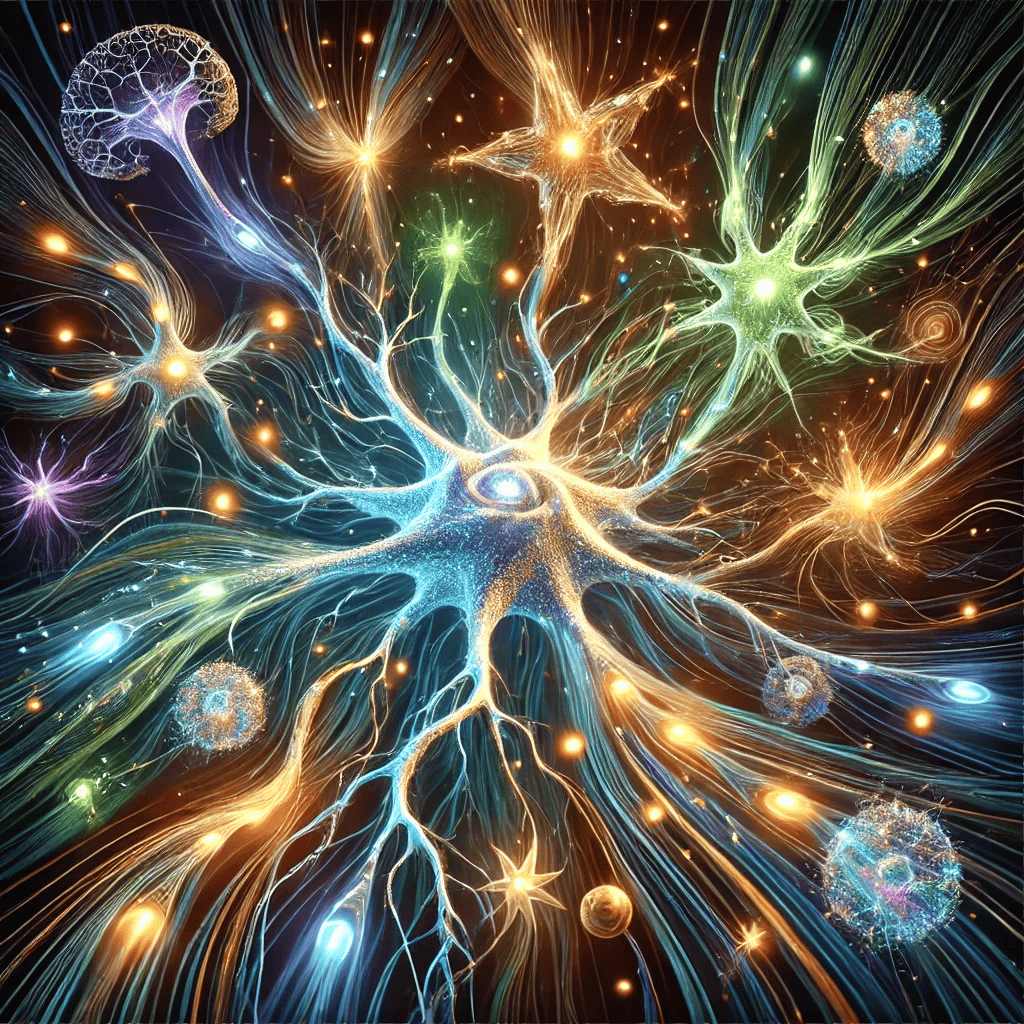
\includegraphics[width=0.8\textwidth]{light_cones.png}

    \caption{Neural light cones as a shorthand for boundary conditions of consciousness}
\end{figure}

The neural light cone concept extends beyond simple spatial and temporal boundaries to encompass the organization of energetic coherence itself. Within each cone, multiple scales of organization—from molecular interactions to regional activation patterns—must maintain alignment to support conscious processing \cite{vazquez2019gradients}. This multi-scale coherence is achieved through triangulation, where different regions within the cone maintain stable relationships through continuous mutual feedback and adjustment.

A key feature of neural light cones is their role in maintaining synchronic and diachronic unity—the integration of conscious experience across space and time respectively. Synchronic unity emerges from the capacity of regions within the cone to achieve simultaneous coherence, while diachronic unity depends on the stable propagation of coherent states across successive temporal windows \cite{tegmark2016improved}. This dual unity is maintained through the continuous operation of feedback loops that stabilize energy flows while allowing for adaptive changes in response to new inputs.

The boundaries of neural light cones are partially determined by thermal noise thresholds, which act as natural limits on the maintenance of coherent energy states \cite{oyama2009noise}. Regions within the cone must maintain sufficient energetic coherence to overcome these thermal fluctuations, while areas that cannot sustain such coherence effectively fall outside the conscious field. This creates a natural selection mechanism for conscious participation, where only those regions capable of maintaining appropriate energetic stability contribute to conscious experience.

Importantly, neural light cones are not isolated structures but form overlapping fields of influence across the cortical sheet. This overlap allows for smooth transitions in conscious experience, as different regions enter and exit the conscious field based on attention, task demands, and metabolic conditions \cite{petermann2009spontaneous}. The interaction between overlapping light cones basically creates a global light cone—a broader field of conscious integration that nonetheless remains bounded by the physical constraints on neural coherence.

The implications of the neural light cone framework extend beyond explaining current conscious experience to inform our understanding of fundamental limitations in consciousness. For instance, the model provides clear reasons why consciousness cannot be "uploaded" or transmitted across arbitrary distances—such processes would necessarily break the continuous, causally-connected energy flows that the light cone maintains \cite{seth2015granger}. Similarly, it explains why consciousness differs fundamentally from sleep states, where energy coherence patterns are altered but not destroyed, versus death, where the capacity for coherent energy maintenance is irreversibly lost.

The neural light cone also helps resolve long-standing questions about the relationship between conscious and unconscious processing. Rather than positing a rigid boundary between conscious and unconscious states, the model suggests a dynamic interface where regions move in and out of conscious awareness based on their ability to maintain coherent energy states within the light cone's boundaries \cite{tononi1998consciousness}. This fluid boundary allows for the brain's remarkable ability to shift attention and integrate new information while maintaining a stable conscious field.

Perhaps most significantly, the neural light cone framework bridges local and global aspects of conscious experience. By describing how local coherence patterns can align and integrate within broader fields of conscious awareness, it provides a physical basis for both the unity and diversity of conscious experience \cite{ramachandran2001synaesthesia}. This integration occurs through mechanisms of mutual recursion and continuous feedback, allowing for coherent diversity—the capacity to maintain distinct local patterns while contributing to a unified global experience.

The implications extend to understanding phenomena such as synaesthesia and other altered states of consciousness, where unusual patterns of integration within the neural light cone may lead to non-typical conscious experiences \cite{abraham1996metaplasticity}. The framework suggests that such phenomena emerge from modifications to the normal boundaries and integration patterns of neural light cones, rather than from purely computational or representational changes.

Understanding how neural light cones enable both local processing and global integration leads naturally to consideration of the temporal dimensions of consciousness—specifically, how the brain maintains both moment-to-moment awareness (synchronic unity) and continuous experience across time (diachronic unity) \cite{hoel2017when}. This theoretical foundation provides a bridge between the physical mechanisms of neural processing and the phenomenological features of conscious experience, suggesting new approaches to investigating both normal and altered states of consciousness.